\section{Tests}
\begin{enumerate}
\item Introduction to the section. What do we want and why. First we want to test A and the X. At last we want to test the complete system.
\item Introduce how we will compare the tests and how we measure the quality -- Mean Squared Error (MSE).
\item Subsection with the error measure
\item Subsection with a introduction to the data sets -- AR and Toy Example data sets.
\item Subsection with the performing of tests
	\begin{itemize}
	\item Talk about the choice for a initial A in the Cov-DL when D is under-complete. Random uniform distribution? or a Gaussian distribution. Show the errors of the real A and estimated A.
	\item With the choice for A we now tests the choice for the number of segmentation in Cov-DL.
	\item Test X with the found A. Make a comparison of the error for X and A in one plot.
	\end{itemize}
\end{enumerate}
With the implemented algorithms -- Cov-DL and M-SBL -- the goal is now to investigate the performance of each algorithm. The performance will be measure by a error measure -- the mean square error (MSE).


\subsection{Error}
To evaluate our baseline algorithm we will perform some test s with knowledge of some real mixing matrices $\mathbf{A}$ and source matrices $\mathbf{X}$ to be compared with our estimated mixing matrices $\hat{\mathbf{A}}$ and source matrices $\hat{\mathbf{X}}$. For the comparison we will look at the differences between the real and estimated matrices. For this task a mean squared error (MSE) method has been chosen. The MSE measure the average squared difference between some estimated value and the actual value. The MSE has the property of always being positive because of the randomness introduced in the method.
The MSE is given by
\begin{align*}
\text{MSE} = \frac{1}{T} \sum_{i=1}^T (G_i - \hat{G}_i)^2,  
\end{align*}
where $T = \{m,n\}$ the numbers of rows of $\mathbf{A}$ or $\mathbf{X}$, $G_i = \{ \mathbf{A}_i, \mathbf{X}_i\}$ is a measurement row of the actual matrix and $\hat{G}_i = \{\hat{\mathbf{A}}_i,\hat{\mathbf{X}}_i\}$ is an estimated row of the estimated matrix.
The MSE is view as a measure of the quality of an estimator, in this case of how M-SBL and Cov-DL perform. 
If the MSE is a large value this implies that the the estimated data values are dispersed widely around its mean while a small MSE value implies that the estimated data is closely dispersed around the mean. Usually, a small MSE value indicate a good estimator but the value cannot be to small as this would indicate that the data has been overfitted. 
A good MSE would be depending on how the data is scattered as wildely scattered data may lead to a MSE not close to zero but it would still be the a good measure for the estimator.


\subsection{Simulation of Data Sets}


\subsubsection{Toy Example}
The first data set which also is the simple and non-realistic data set is used for confirmation that the two presented algorithm work.
The data set is constructed from four different signals: 
\begin{itemize}
\item[-] $\sin(2t)$
\item[-] $\sin(4t)$
\item[-] a sawtooth wave with period $2 \pi t$
\item[-] a sign signal of $\sin(3t)$
\end{itemize}
with $t$ being a time index defined in the interval $[0,10]$ with $L$ samples. Each of the four signal are randomly drawn and used to construct a source matrix $\mathbf{X}$ of size $k \times L$. 
With a source matrix $\mathbf{X}$ a mixing matrix $\mathbf{A}$ of size $M \times k$ is randomly generated from a Gaussian distribution and then normalised. By multiplying the source matrix and the mixing matrix the measurement matrix $\mathbf{Y}$ is achieved and this complete the toy example data set.

An illustration of the data set can be seen in figure \ref{fig:mix}. The data set is constructed for $M = 3$, $k = 4$ and $L = 1000$.
\begin{figure}[H]
\centering
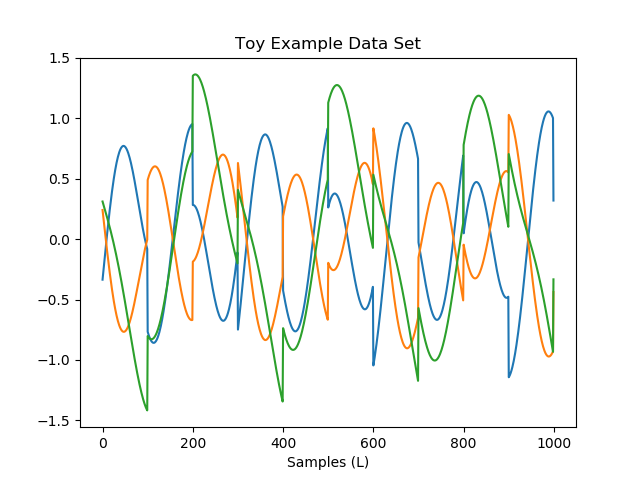
\includegraphics[scale=0.5]{figures/chapter6/Mix_Data_m3_n4_k4_L1000.png}
\label{fig:mix}
\caption{All the signal of the toy example data set for $M = 3$, $k=4$ and $L=1000$.}
\end{figure}
\noindent

\subsubsection{Autoregressive}
The second data set illustrate a more realistic data set.
The data set is constructed from different autoregressive processes: 
\begin{itemize}
\item[-] $\mathbf{x}^{t} = \mathbf{a1}^{t-1} \cdot \mathbf{x}^{t-1} + \mathbf{a1}^{t-2} \cdot \mathbf{x}^{t-2} + \mathbf{w1}_t$
\item[-] $\mathbf{x}^{t+1} = \mathbf{a2}_t \cdot \mathbf{x}_{t-1} + \mathbf{a}_t \cdot \mathbf{x}_t + \mathbf{w}_t$
\item[-] $\mathbf{x}_{t+1} = \mathbf{a}_t \cdot \mathbf{x}_{t-2} + \mathbf{a}_t \cdot \mathbf{x}_t + + \mathbf{a}_t \cdot \mathbf{x}_{t-1} \mathbf{w}_t$
\item[-] $\mathbf{x}_{t+1} = \mathbf{a}_t \cdot \mathbf{x}_t + \mathbf{a}_t \cdot \mathbf{x}_{t-3} + \mathbf{w}_t$
\end{itemize}
with $t$ being a time index defined in the interval $[0,10]$ with $L$ samples. Each of the four signal are randomly drawn and used to construct a source matrix $\mathbf{X}$ of size $k \times L$. 
With a source matrix $\mathbf{X}$ a mixing matrix $\mathbf{A}$ of size $M \times k$ is randomly generated from a Gaussian distribution and then normalised. By multiplying the source matrix and the mixing matrix the measurement matrix $\mathbf{Y}$ is achieved and this complete the toy example data set.

An illustration of the data set can be seen in figure \ref{fig:mix}. The data set is constructed for $M = 3$, $k = 4$ and $L = 1000$.
\begin{figure}[H]
\centering
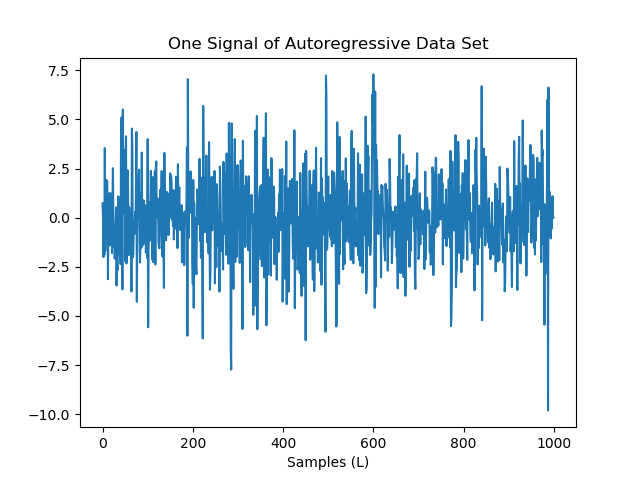
\includegraphics[scale=0.5]{figures/chapter6/AR_Data_m3_n4_k4_L1000.png}
\label{fig:AR}
\caption{All the signal of the toy example data set for $M = 3$, $k=4$ and $L=1000$.}
\end{figure}
\noindent

\subsection{Tests}
INTRODUCTION...


Before any testing of the performance of the algorithms one must test if the algorithm works. The Cov-DL and M-SBL has been tested with the toy example data to see if the algorithms give us a results.

In the following figure we see the recovered sources aligned with the real source of a system with $M = 3$ and $k = 4$ for $L = 100$ -- a small system.
\begin{figure}[H]
\centering
    \begin{minipage}[t]{.45\textwidth}
        \centering
        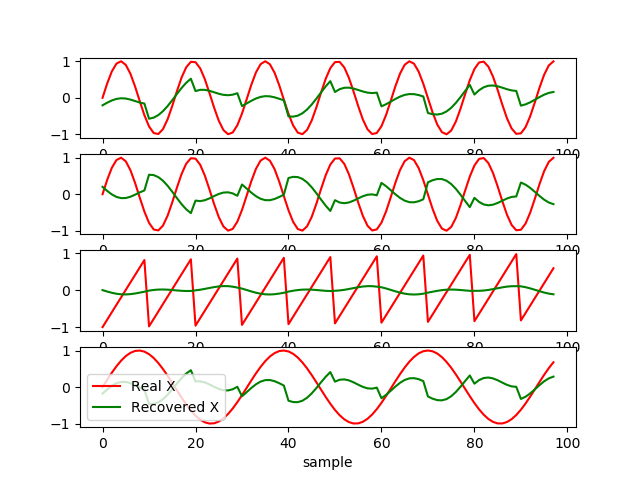
\includegraphics[scale=0.5]{figures/chapter6/test_of_algo_mix_data.png}
\label{fig:test_toy}
\caption{Estimated A}
    \end{minipage} 
    \hfill
    \begin{minipage}[t]{.45\textwidth}
        \centering
        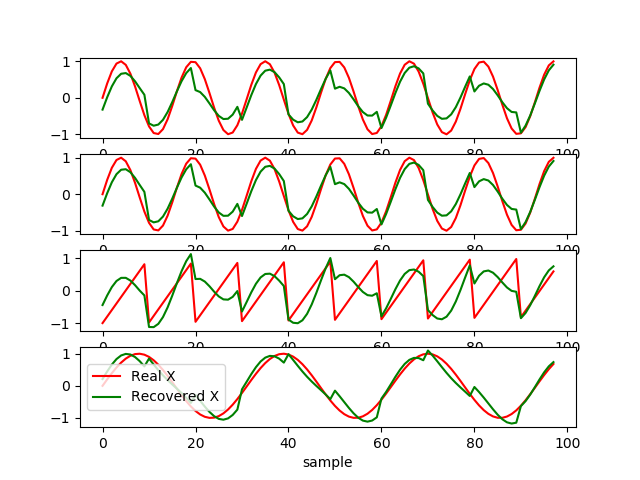
\includegraphics[scale=0.5]{figures/chapter6/test_of_algo_mix_data_realA.png}
\label{fig:test_toy_realA}
\caption{Real A}
    \end{minipage}
\end{figure}
\noindent
Furthermore, if we look at the at the mse then we have a representation error of

\begin{table}[H]
\centering
\begin{tabular}{|c|c|c|}
\hline
         & Estimated A & Real A \\ \hline
MSE of A & 2.23 & $\times$ \\ 
\hline 
MSE of X & 0.53 & 0.14 \\ 
\hline
\end{tabular} 
\caption{Toy Example Data Set}
\end{table}

\subsubsection{Initial A in Cov-DL}
In the Cov-DL algorithm described in XX the over-determined system use the principal component analysis to make an optimization problem from which the matrix $\mathbf{D}$ can be found. To solve the optimization problem and finding $\mathbf{D}$ an initial $\mathbf{A}_{\text{ini}}$ is used as a starting point in the optimization process. The choice of this initial $\mathbf{A}_{\text{ini}}$ will effect how the good an estimate our found mixing matrix $\hat{\mathbf{A}}$ is.

In this section we will be testing three different choice for $\mathbf{A}_{\text{ini}}$:
\begin{itemize}
\item[-] A matrix $\mathbf{A1}$ drawn from a continuous uniform distribution in the half-open interval $[0.0, 1.0)$
\item[-] A matrix $\mathbf{A2}$ drawn from a uniform distribution in the half-open interval $[-1.0, 1.0)$
\item[-] A matrix $\mathbf{A3}$ drawn from a Gaussian distribution with mean 0 and variance 1
\end{itemize}
The test of different initial A's will be performed on the AR data set as this resemble the real data, EEG measurements, at most. The goal with this test is to find the best initial A, with lowest error, such that when the baseline algorithm is used on realistic data, the parameters as been chosen with the best performance in mind -- leading to the best scenario of finding the true mixing matrix and source matrix from EEG measurements.

As the initial A will be used in finding an estimate for the mixing matrix which then be use to finding an estimate of the source matrix, we will look at the performance/error of both Cov-DL and M-SBL to find the best choice in both algorithms.

For the Cov-DL and M-SBL algorithm we are looking at a system of size $M = 8$, $k = 16$ and $L = 1000$. Furthermore, for the Cov-DL the data has been divided in segments of 10 samples.
\begin{table}[H]
\centering
\begin{tabular}{|c|c|c|c|}
\hline 
 & $\mathbf{A1}$ & $\mathbf{A2}$ & $\mathbf{A3}$ \\ 
\hline 
MSE of A & 1.35 & 3.67 & 3.94 \\ 
\hline 
MSE of X & 21.63 & 10.23 & 6.18 \\ 
\hline
\end{tabular} 
\caption{AR Data Set}
\end{table}

\begin{figure}[H]
\centering
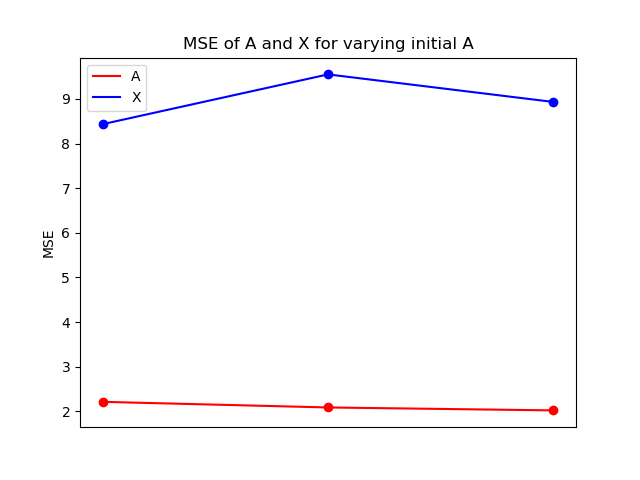
\includegraphics[scale=0.5]{figures/chapter6/AR_Error_initial_A_m8_k16_L1000.png}
\label{fig:initialA_AR}
\caption{}
\end{figure}
\noindent



%\begin{table}[H]
%\centering
%\begin{tabular}{|c|c|c|c|}
%\hline 
% & $\mathbf{A1}$ & $\mathbf{A2}$ & $\mathbf{A3}$ \\ 
%\hline 
%MSE of Cov-DL & 0.70 & 0.66 & 25.99 \\ 
%\hline 
%MSE of M-SBL & 1.07 & 0.78 & 0.72 \\ 
%\hline 
%\end{tabular} 
%\caption{Toy Example Data Set}
%\end{table}
%
%\begin{figure}[H]
%\centering
%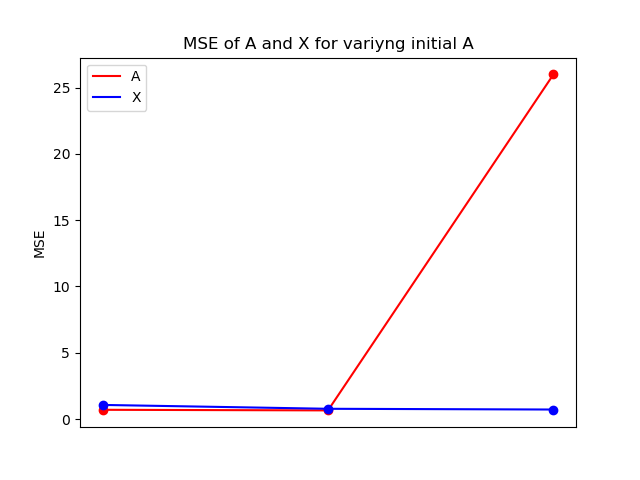
\includegraphics[scale=0.5]{figures/chapter6/Mix_Error_initial_A_m8_k16_L1000.png}
%\label{fig:initialA_mix}
%\caption{}
%\end{figure}
%\noindent


\subsubsection{Segmentation in Cov-DL}
\begin{figure}[H]
\centering
    \begin{minipage}[t]{.45\textwidth}
        \centering
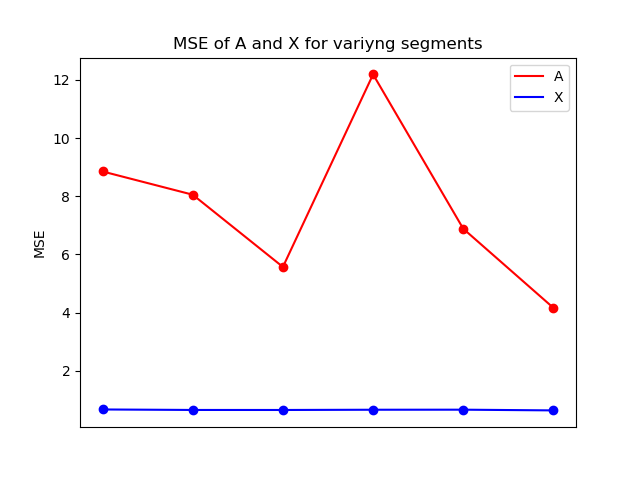
\includegraphics[scale=0.5]{figures/chapter6/Mix_Error_vary_seg_m8_k16_L1000.png}
\label{fig:seg_mix}
\caption{Toy Example Data Set}
    \end{minipage} 
    \hfill
    \begin{minipage}[t]{.45\textwidth}
        \centering
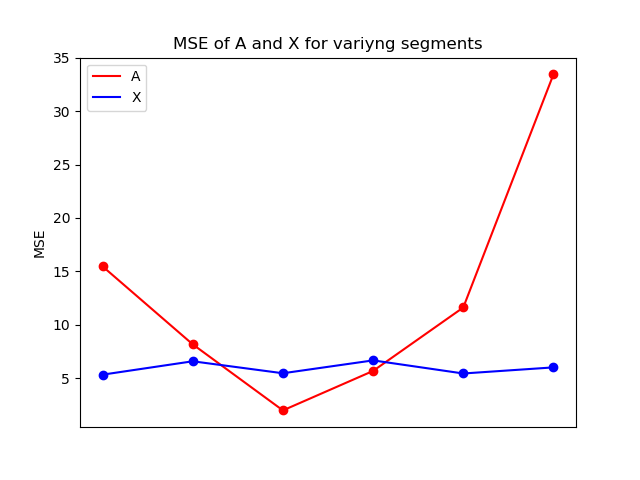
\includegraphics[scale=0.5]{figures/chapter6/AR_Error_vary_seg_m8_k16_L1000.png}
\label{fig:seg_AR}
\caption{AR Data Set}
    \end{minipage}
\end{figure}
\noindent


\begin{table}[H]
\centering
\begin{tabular}{|c|c|c|c|c|c|c|}
\hline 
\textbf{Toy Example Data Set} & & & & & & \\ \hline
 & 10 & 20 & 30 & 40 & 50 & 60 \\ 
\hline 
MSE of A & 8.85 & 8.05 & 5.57 & 12.19 & 6.88 & 4.16 \\ 
\hline 
MSE of X & 0.67 & 0.65 & 0.65 & 0.66  & 0.66 & 0.63 \\ 
\hline
\\ \hline
\textbf{AR Data Set} & & & & & & \\ \hline
 & 10 & 20 & 30 & 40 & 50 & 60 \\ 
\hline 
MSE of A & 15.46 & 8.15 & 1.97 & 5.66 & 11.61 & 33.44 \\ 
\hline 
MSE of X  & 5.31 & 6.57 & 5.45 & 6.65  & 5.42 & 6.00 \\ 
\hline
\end{tabular} 
\caption{Toy and AR Data Set}
\end{table}

